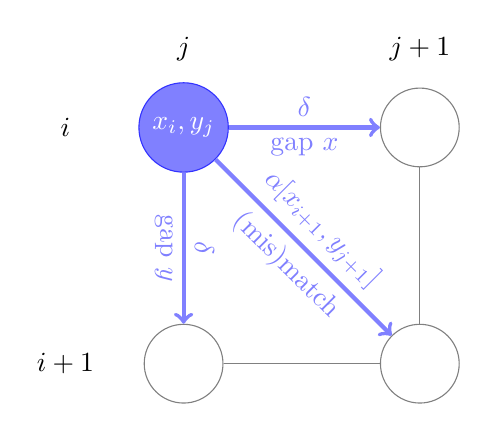
\begin{tikzpicture}
\tikzstyle{strnode}=[circle,draw=gray,minimum width=1cm];
\tikzstyle{move}=[line width=1.5pt, blue!50, ->];
\node[strnode,fill=blue!50,draw=blue!80,font=\color{white}\bfseries] (v1) at (-1,0.5) {$x_i,y_j$};
\node [strnode] (v3) at (2,0.5) {};
\node [strnode] (v4) at (-1,-2.5) {};
\node [strnode] (v2) at (2,-2.5) {};
\draw [move] (v1) edge node[sloped,above] {$\alpha[x_{i+1},y_{j+1}]$} node[sloped,below] {(mis)match} (v2);
\draw [gray] (v3) edge (v2);
\draw [gray] (v4) edge (v2);
\draw[move] (v1) edge node[sloped,above] {$\delta$} node[sloped,below] {gap $x$} (v3);
\draw[move] (v1) edge node[sloped,above] {$\delta$} node[sloped,below] {gap $y$} (v4);
\node at (-2.5,0.5) {$i$};
\node at (-2.5,-2.5) {$i+1$};
\node at (2,1.5) {$j+1$};
\node at (-1,1.5) {$j$};
\end{tikzpicture}